\chapter{System Architecture}


\begin{figure}
  \centering
  %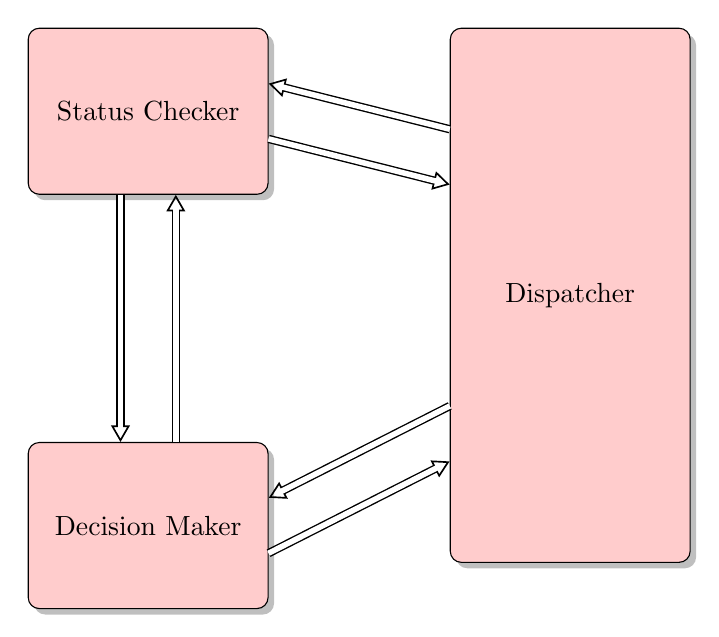
\begin{tikzpicture}
  \usetikzlibrary{arrows, shadows, decorations.markings}
  \tikzstyle{vecArrow} = [thick, decoration={markings,mark=at position
	1 with {\arrow[semithick]{open triangle 60}}},
	double distance=1.4pt, shorten >= 5.5pt, preaction = {decorate},
	postaction = {draw,line width=2pt, white,shorten >= 4.5pt}
  ]
  \tikzstyle{component} = [draw,text centered,rounded corners,drop
  shadow,text width=8em,fill=red!20,minimum height=6em]
  \tikzstyle{dispatcher} = [component,minimum height=19.3em]

  % Define distances for bordering
  \def\blockdist{2.3}
  \def\edgedist{2.5}

  % Draw components
  \node[component](status-checker){Status Checker};
  \path (status-checker.north east)+(\blockdist,0) node[dispatcher, anchor=north west](dispatcher){Dispatcher};
  \path (status-checker.south)+(0,-4.2) node[component](decision-maker){Decision Maker};
  \draw[vecArrow] ([xshift=-10]status-checker.south) to ([xshift=-10]decision-maker.north);
  \draw[vecArrow] ([xshift=10]decision-maker.north) to ([xshift=10]status-checker.south);

  %Draw interaction arrows
  \def\composhift{50}
  \draw[vecArrow] ([yshift=-10]status-checker.east) to ([yshift=-10+\composhift]dispatcher.west);
  \draw[vecArrow] ([yshift=10+\composhift]dispatcher.west) to([yshift=10]status-checker.east);

  \draw[vecArrow] ([yshift=-10]decision-maker.east) to ([yshift=-10-\composhift]dispatcher.west);
  \draw[vecArrow] ([yshift=10-\composhift]dispatcher.west) to ([yshift=10]decision-maker.east) ;
\end{tikzpicture}

  \usetikzlibrary[backgrounds]
\begin{tikzpicture}
  \node[](key-comp){\begin{tikzpicture}
  \usetikzlibrary{arrows, shadows, decorations.markings}
  \tikzstyle{vecArrow} = [thick, decoration={markings,mark=at position
	1 with {\arrow[semithick]{open triangle 60}}},
	double distance=1.4pt, shorten >= 5.5pt, preaction = {decorate},
	postaction = {draw,line width=2pt, white,shorten >= 4.5pt}
  ]
  \tikzstyle{component} = [draw,text centered,rounded corners,drop
  shadow,text width=8em,fill=red!20,minimum height=6em]
  \tikzstyle{dispatcher} = [component,minimum height=19.3em]

  % Define distances for bordering
  \def\blockdist{2.3}
  \def\edgedist{2.5}

  % Draw components
  \node[component](status-checker){Status Checker};
  \path (status-checker.north east)+(\blockdist,0) node[dispatcher, anchor=north west](dispatcher){Dispatcher};
  \path (status-checker.south)+(0,-4.2) node[component](decision-maker){Decision Maker};
  \draw[vecArrow] ([xshift=-10]status-checker.south) to ([xshift=-10]decision-maker.north);
  \draw[vecArrow] ([xshift=10]decision-maker.north) to ([xshift=10]status-checker.south);

  %Draw interaction arrows
  \def\composhift{50}
  \draw[vecArrow] ([yshift=-10]status-checker.east) to ([yshift=-10+\composhift]dispatcher.west);
  \draw[vecArrow] ([yshift=10+\composhift]dispatcher.west) to([yshift=10]status-checker.east);

  \draw[vecArrow] ([yshift=-10]decision-maker.east) to ([yshift=-10-\composhift]dispatcher.west);
  \draw[vecArrow] ([yshift=10-\composhift]dispatcher.west) to ([yshift=10]decision-maker.east) ;
\end{tikzpicture}
};
  \begin{pgfonlayer}{background}
  	%\node[text centered,minimum width=4em,rounded corners,fill=yellow!25]{};
	\node[draw,dashed,rounded corners,fill=yellow!30](management) {Management System} ;
	%(key-comp.north west) rectangle (key-comp.south east);
  \end{pgfonlayer}
\end{tikzpicture}


  \caption{System Architecture Overview}
  \label{fig:archi-overview}
\end{figure}

Figure~\ref{fig:archi-overview} shows the architecture of this cloud
management system, which consists of three components: \emph{Status
Checker}, \emph{Decision Maker} and \emph{Dispatcher}.  The management
system can form a complete cloud computing system by connecting with a
number of \emph{workers} or work as a part of existent cloud systems.

We implemented components and the worker as separate RPC (remote
procedural call) servers.  Separate RPC server implementation makes each
component \emph{pluggable}.  The pluggability gives the system
administrator flexibility to choose the most suitable component
implementation to fit different needs.  Moreover, without shutting the
whole system down, we can change system configurations, or even upgrade
the system,  by substituting target components with feasible ones.
Besides, this design allows us to easily integrate the management system
with other cluster management systems like JPPF~\cite{cite:JPPF}.
Roystonea~\cite{cite:roystonea} also benefits from the RPC server
implementation.




\section{Worker}

Workers are the ones using resource of the cloud directly.  They execute
tasks assigned by the management system.  A worker instance executes at
most one task at a time, but it doesn't mean that a physical machine can
run one task only at a time.  One can run multiple worker instances on a
physical machine so that a physical machine could run more than one task
simultaneously.	 

Deploying multiple worker instances on a powerful machine (e.g., with
large number of cores) can gain better performance from
multiprogramming, but in contrary, it might however cause resource
contention on low-end machines.  We leave the choice to system
administrators.  If the task execution performance of a machine running
multiple worker instances is far worse than expected, it is very likely
due to resource contention.  In that case, the system administrator
should consider reducing the number of worker instances on that machine.
Thanks to the pluggable implementation, this can be done \emph{online},
without stopping any of other components, even running workers we'd like
to keep on that machine, by simply stop several worker instances.

% Possibly move this to other section???
In fact, our management system can function without workers.  In the
case that it is working as a part of other cluster management systems,
the system in charge is instead responsible for manipulating physical
resources.

\section{Status Checker}

Status checker periodically collects the information about physical
servers, including the server status and its resource usage.  A physical
server can be in status of either \emph{available}, \emph{occupied},
\emph{busy} or \emph{down}.
% TODO  Talk about states
Such information is provided to the decision maker as reference
for making allocation adjustment.  

\section{Decision Maker}

Decision maker is in charge of making and adjusting resource
allocation plans according to the specified policy that takes different
parameters such as job deadline and priority into consideration. It is
designed to be in \emph{passive mode}, which means it is invoked (by the
dispatcher) only under certain circumstances (which will be discussed
later) rather than periodically schedules resources by itself.

\section{Dispatcher}

Dispatcher is the component that deal with the physical resource
allocation adjustment according to the allocation plan made by the
decision maker.

\section{Work Flow}

